\documentclass{article} % For LaTeX2e
\usepackage{nips13submit_e,times}
\usepackage{hyperref}
\usepackage{url}
\usepackage{graphicx}
\usepackage{wrapfig}
\usepackage{caption}
\usepackage{subfig}

\captionsetup{
  font=footnotesize,
  justification=raggedright,
  singlelinecheck=false
}

\title{Banishing the Bid Bot: Detecting Online Bidding Fraud in Facebook Auctions \\ \large Team Random Clique}

\author{
Daniel Geng \\
504588536 \\
Department of Computer Science\\
University of California, Los Angeles\\
\texttt{xpdaniel2@gmail.com} \\
\And
Meghana Ginjpalli \\
804588573 \\
Department of Computer Science \\
University of California, Los Angeles\\
\texttt{mginjpalli@ucla.edu} \\
\AND
Sara Melvin \\
004590481 \\
Department of Computer Science \\
University of California, Los Angeles\\
\texttt{sara.melvin@gmail.edu} \\
\And
Sonu Mishra \\
604590548 \\
Department of Computer Science\\
University of California, Los Angeles\\
\texttt{mishrasonu1993@gmail.com} \\
\And
Andrew Wong \\
104036702 \\
Department of Computer Science\\
University of California, Los Angeles\\
\texttt{anjuwong@ucla.edu} \\
}

\newcommand{\fix}{\marginpar{FIX}}
\newcommand{\new}{\marginpar{NEW}}

\nipsfinalcopy % Uncomment for camera-ready version

\begin{document}

\maketitle

\begin{abstract}

stuff

\end{abstract}

\section{Motivation}

Facebook is a popular online social media platform connecting users from all around the world.
Because of its high traffic, Facebook is an ideal form of commercial advertisement.
Businesses are able to reach out to their existing customers as well as advertise to new customers by specifying which group of users they would like to advertise to.
Although Facebook can provide space on both their website and mobile site, there is limited webpage ``real estate".
Therefore, Facebook sets up auctions for businesses to bid on designated spaces for advertisement purposes.

Online shopping and bidding are quickly becoming a major proportion of retail transactions. \cite{shopping}
Consumers are increasingly enjoying the convenience and selection provided by the e-commerce platforms available today.
Unfortunately, legitimate users are being frustrated by bots as they bid at the last possible second.
Automated bids from bots are unfairly able to submit bids almost instantaneously, making it difficult for legitimate buyers to win auctions.
According to a paper released by eBay, 65\% of sessions each day are initiated by bots. \cite{ebay}

``Facebook Recruiting IV: Human or Robot?" was a past Kaggle Competition that ended in June 2015.
The competition tackles the problem of bot detection in Facebook Ads bidding.
Our goal is to detect bot-user anomalies in this e-commerce environment using various anomaly detection methods.

\section{Background}

Existing approaches have been implemented in order to determine pattern detection for identifying anomalous users.
There are many platforms relying on crowdsourcing for promoting products and services.
However, there are bots pretending to be humans which lowers the consumers' trust in these sites.
Thus, there is a lot of motivation for these companies to have some type of anomaly detector for removing these bots.
These approaches are group-based, temporal-based, and edge attribute graph-based.

\subsection{Group-based Approach}

This approach aims to detect groups of anomalies based on features across multiple users.
Previous methods have attempted to classify based on the similarity of feature groups. \cite{ndsync}
Other methods detect group based anomalies by determining groups based on closeness of certain features, and then determining which groups are anomalous. \cite{glad}
The benefits of using these group-based approaches is that it uses the sheer amount of data provided to its advantage.
Generally, however, these approaches assume a static model for the data.
Additionally, due to the large amount of data processed by these approaches, the methods are computationally expensive.

\subsection{Temporal-based Approach}

Unlike some of the other approaches, this method uses only one feature to detect bot-users? suspicious activity.
The temporal-based approach operates under the assumption that the time between user events for bots is significantly different behavior than normal users. \cite{birdnest} \cite{rsc} \cite{sfp} \cite{cicp}
This assumption holds in most situations.
However, bots could be compromised users, which camouflages the anomalous temporal feature(s) with their human host.
Therefore, other features may need to be used for improved detection of bot-users.

\subsection{Edge-attributed Graph-based Approach}

Conventional graph-based approaches observe topological patterns of relations between entities (i.e. users, products, etc), but do not leverage the edge-attributes.
The algorithm proposed in EdgeCentric utilizes more features by representing the relationship between entities as an edge-attributed multigraph. \cite{edgecentric}
Given the distribution of various clusters of benign user behavior, the information required to describe the behavior of a new user is found in terms of its minimum description length (MDL) from the clusters.
The MDL is used to compute how suspicious a certain user is.
The strength of this approach, however, relies on the rating relationship between users, products, and buyers.
In the project?s bidding data, a seller and rating information is not disclosed, which potentially weakens the applicability of this approach.

\section{Methods}

Various anomaly detection algorithms are compared and contrasted, including BIRDNEST, EdgeCentric and classic machine learning algorithms such as K-means, logistic regression, kernel SVM, naive Bayes, and decision trees to discover bot-anomalous behavior.
Additionally, these models are compared to the model implemented by the winner of this Kaggle Competition, Small Yellow Duck.
Because the dataset from Kaggle (\url{https://www.kaggle.com/c/ facebook-recruiting-iv-human-or-bot/data}) provides labeled data, we are focusing on using supervised algorithms for detection.
We plan to use k-fold cross validation and tune our hyperparameters evaluation metrics. 

To evaluate the efficacy model, we will apply the trained model to our testing data and compare the classifying algorithms based on performance.
The metrics we will use to evaluate the performance of our algorithms is the area under the ROC curve (AUC). 

\section{Data}

The data provided includes timestamps of bids, merchandise categories, bidding devices, countries of bids, and the reference URL for a bid.
We plan to use these features and state-of-the art anomaly detection algorithms to determine which method will best identify bot-users.

The bidder dataset contained approximately 2,000 instances and had the following features: bidder\_id, payment\_account, address, outcome.
The bid dataset contained approximately 7.6 million instances and had the following features: bid\_id, bidder\_id, auction, merchandise, device, time, country, ip, url.

The training data set provided by Kaggle had labels for each user, classifying each individual as a human or a bot.
However, the testing data had no labels; therefore, only the training data set could be used for training, validation, and testing.

The training data set was joined with the bids data set, resulting in over 3 million bids.
Overall, it contained 1,984 distinct bidders with 103 of the total users classified as bots.

\section{Software Tools}

Python was used for a majority of our data processing, given the large number of libraries that are publicly available.
Sklearn has a number of built-in machine learning algorithms.
Numpy is very useful for working with matrices and different feature vectors.
Pandas has a high performance data analysis tool used to analyze large amounts of data.
Matplotlib facilitates data visualization, which will yield insights into how our data are related.
Additionally, Python has APIs for Apache Spark and Hadoop, which may prove useful for large-scale data processing.

\section{Results}

\subsection{Kaggle Winner: ``Small Yellow Duck"}

The second place winner of this Kaggle Competition is a professional data scientist and goes by the name ``Small Yellow Duck".
Her classification model takes the average of the probabilities predicted by five instances of the Random Forest Classifier, which is an ensemble learning method that constructs multiple decision trees to create a stronger classification model.

Small Yellow Duck first makes a couple of observations before implementing feature extraction.
First, human bidding activity tends to peak daily as seen in the figure below.
Over the course of three days, there are three peaks where human bidding activity is higher.
This may be because of auctions ending at the same time everyday.

\begin{figure}[h]
\centering
\captionbox{Daily peaks of human bidding activity}{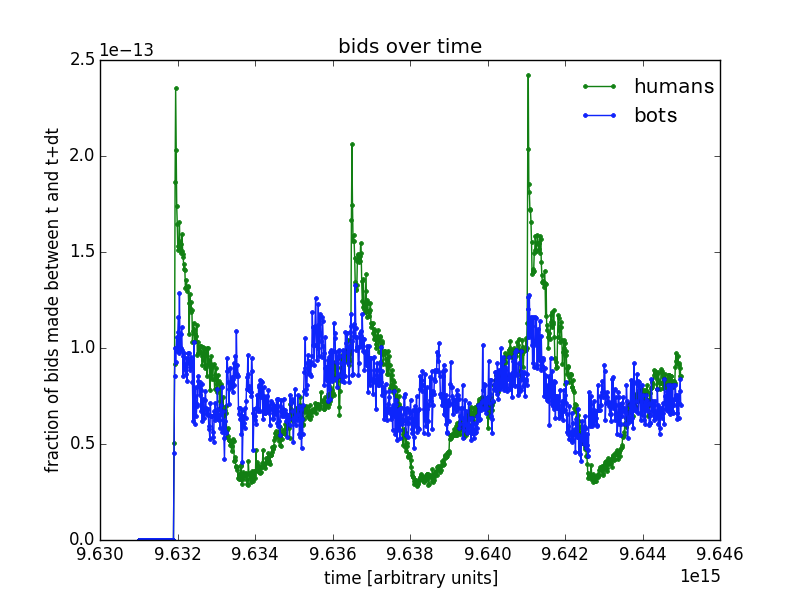
\includegraphics[scale=0.26]{img/yellowduck1.png}}
\end{figure}

Another observation that she made is that auctions tend to last for longer than two weeks.
In this timeframe, robots do not place any bids between 11 to 14 days before the auction ends.
In the figure below, the auction runs for approximately 17 days.
For some reason, between days 11 and 14, human bidding commences while bots tend to keep silent in this duration.

\begin{figure}[h]
\centering
{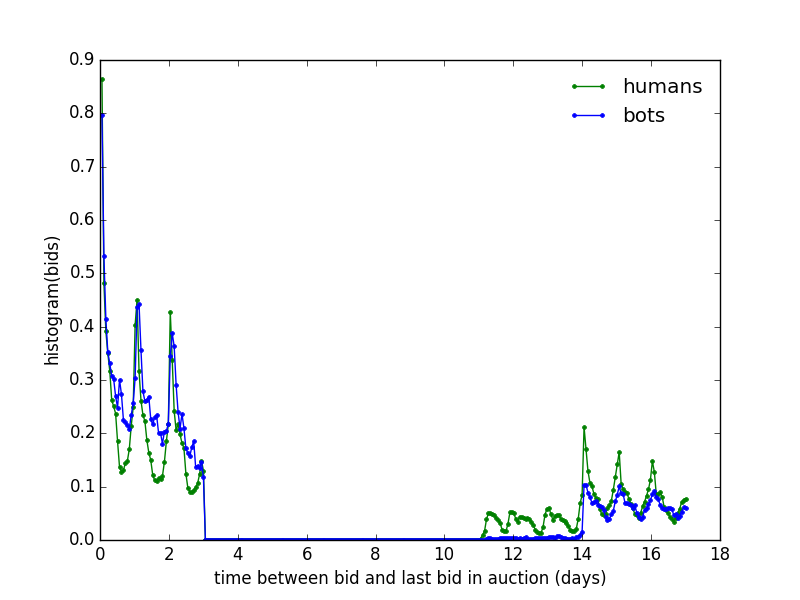
\includegraphics[scale=0.26]{img/yellowduck2.png}}
\end{figure}

During feature extraction, Small Yellow Duck was able to extract the following features: the median time between user's bid and user's previous bid, the mean number of bids a user made per auction, entropy for how many bids a user placed on each day of the week, max number of bids in a 20 min span, total number of bids placed by user, average number of bids a user placed per URL, number of bids placed by the user on each of three weekdays in the data, and min and median times between a user's bid and previous bid by another user in the same auction.

In order to evaluate her results, Small Yellow Duck does cross validation with 100 different training and validation splits where 80\% was training data and 20\% was validation data.
In terms of runtime, training and predicting takes around 3 minutes while 100-fold cross validation takes around 20 minutes.
As a result, the AUC score tends to average at 0.94167. Based on her AUC score, our highest performing algorithm would allow us to be in the top 15\% of the leaderboard.

\subsection{Classic Machine Learning Approaches}

All machine learning models were implemented for binary classification, rather than a suspiciousness score.
Initially, support vector machines (SVMs) and logistic regression were implemented.
SVMs were tested with linear, polynomial, and radial kernels and logistic regression was tested using both primal and dual optimization functions.

However, because these models alone were not very effective, a myriad of boosting and ensemble methods were used in an attempt to improve performance.
The following methods were tested:

\begin{itemize}
\item Adaboost -- weights each classifier based on performance
\item Gradient boosting -- fits trees based on negative gradient of loss function
\item Random forests
\item Bagging -- trains on subsets of data and uses them to vote
\item Extra trees -- trains on subsets of data and averages them
\end{itemize}

All of these models fit numerous classifiers---typically decision trees---to make up for the shortcomings of the earlier classifiers.

\subsubsection{Features}

The given data was pre-processed in various ways.
A combination of the following features were tested in each model to varying degrees of performance.

\begin{itemize}
\item Log-bucketed IAT (base 2 and base 5) -- each bucket is a feature
\item Log-bucketed response time (base 2 and base 5) -- each bucket is a feature
\item Mean IAT
\item Mean response time
\item Total number of bids
\item Mean bids per auction
\item Number of devices
\item Number of IPs
\item Entropy of devices
\item Entropy of IPs
\end{itemize}

\subsection{BIRDNEST}

BIRDNEST is a Bayesian-based approach to anomaly behavior detection.
This algorithm identifies anomalous users by generating a mixture model of given user behavior distributions (BIRD model) and then calculates a user?s score by taking the negative log likelihood the user?s distribution would be generated by the mixture model (NEST metric).
Originally, the algorithm was built to identify rating-fraud by observing two features: rating behavior and inter-arrival times between user activity.
In the context of auction bidding, the rating behavior was not used, but the temporal feature aspect of the algorithm seemed similar to the given situation.
Therefore, this algorithm was chosen and adjusted to be a temporal-based approach.

The hypothesis was that bot bidders would be similar to bot reviewers; bots would bid many times in a very short amount of time and not show the heavy-tail distribution of long spans of time of inactivity common to most human users.
In addition, if a certain master of a bot was watching certain auctions, then whenever a user made a bid on the auction, the bot would quickly make another bid.
The idea was that the bot would make the bid so quick that it would show a distinct response time distribution from human users.
Therefore, inter-arrival time (IAT) and response time were the features that we utilized.

\subsubsection{Features}

\begin{enumerate}
\item IAT distribution -- time between a user's activity events
\item Response time -- time between the previous bidder's bid and the user
\end{enumerate}

\subsubsection{Testing Methodology}

To test which features contribute the most, this algorithm was tested with just IAT as the only feature and then with both IAT and response time as features.
This approach does not split up data in the usual testing/training data set to do cross validation.
However, the BIRD mixture model is calculated by taking a subset of each cluster?s user distributions to estimate optimal hyperparameters.

Since the BIRD model takes random subsamples to optimize parameters, it resulted that varying the K parameter of the number of clusters did not always benefit or decrease the algorithms performance.
Therefore, the algorithm was run for 1 cluster to 20 clusters.
Each user?s score was averaged and then re-ranked from highest to lowest.
Then, true positive rate and false positive rate were calculated to create the ROC curve.
Algorithm performance was measured by the area under the curve (AUC) of the final ROC curve.

\subsubsection{Assumptions}

For the testing, the following assumptions were made:

\begin{itemize}
\item There were over 40,000 users (majority human) that made a bid with the same username on the same auction at the same time from a different IP address.
This was assumed to be a company having multiple people watching the auctions and placing bids; therefore, the duplicate entry was removed.
\item All users that did not have more than one bid in the data set were given zero IAT distributions.
\item All bids that initiated the auction and all bids that were made by the same bidder at the same auction at the same time were not binned in the response time buckets.
At first, these were considered zero, but upon testing it was found that ignoring them would lead to similar results.
\item Response time used is a reflection of the Kaggle winner?s response time feature, except the distribution is utilized in this approach while the Kaggle participant used the median as a feature.
\end{itemize}

\subsubsection{Results: IAT only}

Using only IAT distributions as the feature, the algorithm did not perform as well as some of the classic machine learning classification algorithms.
The figure below shows the ROC with an AUC of only 0.8415.

\begin{figure}[h]
\centering
{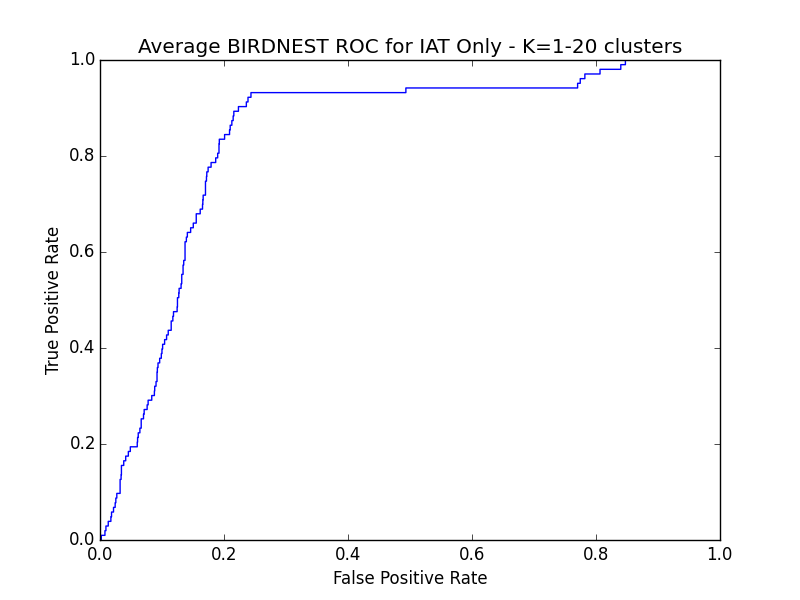
\includegraphics[scale=0.47]{img/bird_iat_roc.png}}
\end{figure}

Upon looking closer at the consistently top anomalous users, it became more clear why this feature did not work very well.
There are many users that are classified as human but show obvious signs of being more than one person.
This means that their IAT distributions are even more suspicious than bots.
For example, one user bid over 500,000 times in the 3 day intervals of the 3 weeks given in the data set.
Many of those bids were duplicates where the bidder would be bidding on the same auction at the same time but from different IP addresses.
In addition, this user (and many users like this one who had many active people behind one username) showed a large amount of small IATs which was hypothesized as only a bot-behavior characteristic.

From visualizing the distributions in the figure below, these features are not nearly as distinct as originally thought.

\clearpage

\begin{figure}[h]
\centering
{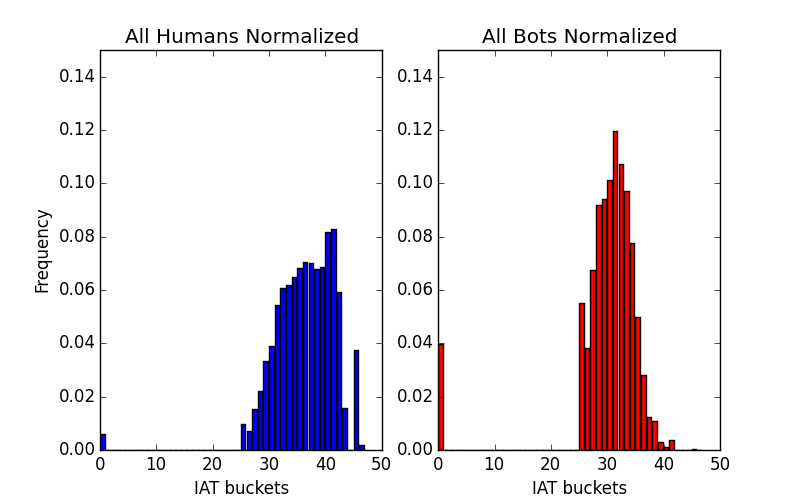
\includegraphics[scale=0.5]{img/bird_iat_dist.png}}
\end{figure}

This algorithm produced the following distributions for its predicted classification of ``normal" and ``robot" users (see figure below).
While the algorithm is able to identify the bot behavior, there are also many human users with similar behavior patterns.

\begin{figure}[h]
\centering
{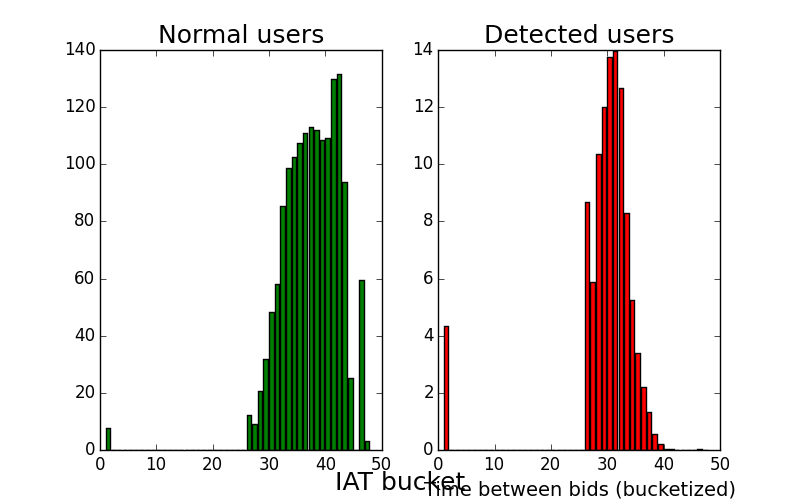
\includegraphics[scale=0.5]{img/bird_iat_pred.png}}
\end{figure}

\subsubsection{Results: IAT and Response Time}

Using Response Time and IAT distributions as features, the performance was only marginally improved.
The figure below shows the ROC with an AUC of 0.8456.

\clearpage

\begin{figure}[h]
\centering
{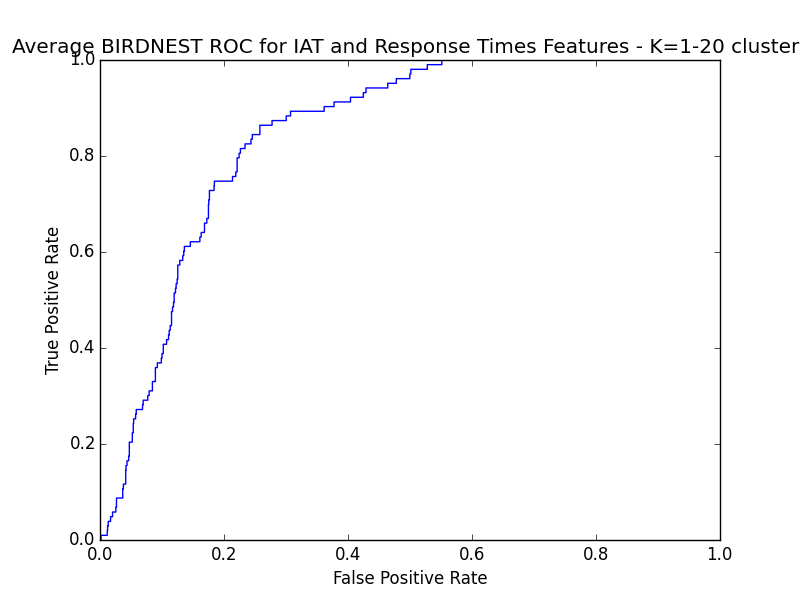
\includegraphics[scale=0.47]{img/bird_roc.png}}
\end{figure}

Upon visualizing the response time distributions for the true bots and benign users, there is practically no difference between the aggregated distributions (see figure below).
As can be seen, there is no major distinction of anomalous when utilizing this feature and was not necessary to add.

\begin{figure}[h]
\centering
{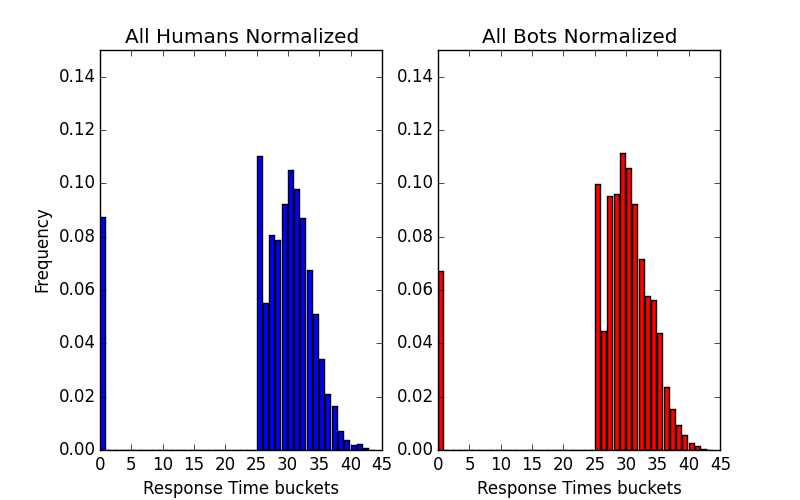
\includegraphics[scale=0.5]{img/bird_res_dist.png}}
\end{figure}

\section{Discussion}
In conclusion, we started this project trying to compare and contrast different algorithms and features to see which one would perform better. In the end, our results were actually comparable to the Kaggle winner's approach. The optimal algorithm turned out to be Gradient Boost and other boosted machine learning approaches. \\

From this project, we gained a few takeaways and future direction. First of all, manipulating a lot of data can be difficult but using the right tools, finding the right features, organizing or sorting it before hand, or storing them as binaries make a huge difference. Secondly, temporal features are not nearly as powerful as we originally though. Once we added entropy terms and different metrics for the number of resources each user was using to bid, we did see dramatic improvement. Although our results are comparable, we could improve these scores by extracting more interesting features that would lead to an improvement of accuracies. Furthermore, as ?state-of-the-art? as certain algorithms are, we should never underestimate the power of numbers. Combining multiple estimators through different boosting methods allows an estimator to fill in the gaps where another estimator might fail, making for a much more powerful classification algorithm. Although boosting the algorithms greatly improves performance, we would have liked to seen if there was a singular algorithm that is just as powerful on its own without taking too much training time. Also, we did attempt a group-based and graph-based approach to apply to our data set but the scalability proved to be a huge issue and made it difficult to debug in the time we needed for this project and was not scalable in preprocessing data into a graph. In conclusion, we learned quite a lot of interesting ways to manipulate large amounts of data and get important features out of this. In addition, we were able to determine what types of algorithms performed better than others.


\section{Contributions}

Daniel: Most of report

Meghana: Presentation, Kaggle winner code/writeup, References

Sara: BIRDNEST, Presentation, References

Sonu: Presentation

Andrew: Machine learning code, Presentation

\begin{thebibliography}{123}

\bibitem{shopping} ``15 Mind-Blowing Stats About Online Shopping." 15 Mind-Blowing Stats About Online Shopping.
\bibitem{ebay} Zhao, K. and Pengju, Y. ``Machine Learning Method In eBay Bot Detection." Ebay Tech Blog. September 4 2014.
\bibitem{ndsync} Giatsoglou, M. et. al. ``ND-Sync: Detecting Synchronized Fraud Activities." Advances in Knowledge Discovery and Data Mining, 2015, 201-214t
\bibitem{glad} Qi, Y., Xinran He, and Yan Liu. ``GLAD: Group Anomaly Detection in Social Media Analysis- Extended Abstract." arXiv:1410.1940.
\bibitem{birdnest} Hooi, B., et. al. ``BIRDNEST: Bayesian Inference for Ratings-Fraud Detection." arXiv:1511.06030
\bibitem{rsc} Costa, A.F. et. al. ``RSC: Mining and Modeling Temporal Activity in Social Media." Proceedings of the 21th ACM SIGKDD International Conference on Knowledge Discovery and Data Mining, 2015, pp. 269-278
\bibitem{sfp} Vaz de Melo, P. et. al. ``The Self-Feeding Process: A Unifying Model for Communication Dynamics in the Web." Proceedings of the International Conference on World Wide Web (WWW), pp. 1319?1330, 2013.
\bibitem{cicp} Malmgren, M.D. et. al. ``Characterizing Individual Communication Patterns." Proceedings of the 15th ACM SIGKDD International Conference on Knowledge Discovery and Data Mining, 2009, pp. 607?616.
\bibitem{edgecentric} Shah, N. et. al. ``EdgeCentric: Anomaly Detection in Edge-Attributed Networks." arXiv:1510.05544.

\end{thebibliography}

\end{document}